% A template for an Honours Thesis in English Language, NUS: adapted from one by Derek Lim (2016), itself adapted from a template for Carleton College comps papers by Andrew Gainer-Dewar (2013). 
% This work is licensed under the Creative Commons Attribution 4.0 International License.
% To view a copy of this licence, visit http://creativecommons.org/licenses/by/4.0/ or send a letter to Creative Commons, 444 Castro Street, Suite 900, Mountain View, California, 94041, USA.
\documentclass[twoside]{memoir}
\usepackage{nus-el-ht}

% The Latin Modern font is a modernised replacement for the classic Computer Modern. Feel free to replace this with a different font package.
\usepackage{lmodern}
% Hyperref enables click-through hyperlinks in your PDF. The hyphens option indicates where to break long URLs. 
\PassOptionsToPackage{hyphens}{url}\usepackage{hyperref}
% We use setspace to implement double-spacing, but with a specific command to leave quotes single-spaced. 
\DisemulatePackage{setspace}\usepackage{setspace}
\expandafter\def\expandafter\quote\expandafter{\quote\singlespacing}
	\doublespacing

% tikz stuff
\usepackage[usenames,dvipsnames]{color}    
\usepackage[table]{xcolor}
\usepackage{themecolors}
\usepackage{tikz} 
\usetikzlibrary{positioning, shapes.multipart, arrows, arrows.meta, shadows, backgrounds, fit}

% code blocks
\usepackage{listings}
\lstdefinelanguage{isabelle}{%
    keywords=[1]{type_synonym,datatype,fun,abbreviation,definition,proof,have, using, thus, lemma,theorem,session,sessions,theories,text,section,inductive},
    keywordstyle=[1]\bfseries\color{isabelleouterblue},
    keywords=[2]{where,assumes,shows,and},
    keywordstyle=[2]\bfseries\color{isabelleoutergreen},
    keywords=[3]{if,then,else,case,of,SOME,let,in,O},
    keywordstyle=[3]\color{isabelleinnerblue},
    keywords=[4]{apply, by, done},
    keywordstyle=[4]\color{isabelleoutersalmon},
    morestring=[b]",
    morecomment=[n]{(*}{*)},
    % morecomment=[n]{\guilsingleft}{\guilsingright},
    stringstyle=\color{isabellequote},
    showstringspaces=false,
}
\lstdefinelanguage{file}{
}
\lstdefinestyle{tree}{
literate=
    {├}{{\smash{\raisebox{-1ex}{\rule{1pt}{\baselineskip}}}\raisebox{0.5ex}{\rule{1ex}{1pt}}}}1 
    {└}{{\smash{\raisebox{0.5ex}{\rule{1pt}{\dimexpr\baselineskip-1.5ex}}}\raisebox{0.5ex}{\rule{1ex}{1pt}}}}1 
    {─}{{\raisebox{0.5ex}{\rule{1.5ex}{1pt}}}}1 
    {│}{{\smash{\raisebox{-1ex}{\rule{1pt}{\baselineskip}}}\raisebox{0.5ex}{\rule{1ex}{0pt}}}}1 
}
\lstset{%
  language=isabelle,
  escapeinside={&}{&},
  columns=fixed,
  extendedchars,
  basewidth={0.5em,0.45em},
  basicstyle=\ttfamily,
  mathescape,
  frame=single,  % adds a frame around the code
}
\lstnewenvironment{nlisting}{\lstset{numbers=left}}{}


% For typesetting and labelling examples, incl. glossed examples. 
% \usepackage{expex} 
% 	\lingset{Everyex=\singlespace}

% Titling commands. 
\title{Stacking Correspondence: Towards Formal Verification of a Network Stack}
\author{Daniel Neshyba-Rowe}
\supervisor {Alain K{\"a}gi}
\degree{Bachelor of Arts with Honors}
\faculty{Mathematical Sciences faculty} % TODO: figure out if this is right
\dept{Computer Science} % TODO: should this be CS and Math?
% \date % TODO: set date?

\begin{document}
% First, we go into "front matter" mode.
% Among other things, this gives us Roman page numbers.
\frontmatter

% We tell LaTeX to make a title page, sections for acknowledgements, the abstract, and the table of contents (important!). 

\maketitle

\chapter{Acknowledgement}
`This page is for making acknowledgements that have a direct bearing on the HT and is not for indulging in routine gestures of politeness or sentimental attitudinising. In all things, the candidate should be guided by good taste and good sense' \pgcitep{data-refinement}{2}. % Note also the command for citing a source and a page number. 

\begin{abstract}
  % citations look like \citep{ell-ht-format}.
      %   Prior work led to the first proven-reliable and viable microkernel, seL4.
      % We hypothesize that similar reliability is possible for a performant IoT device.
      % As a proof of concept, we are creating a networked fish tank thermometer
      % with a complete IPv6 network stack and formally verifying all components.
      %
      % \begin{itemize}
      %     \item should be written for a more general audience
      %     \item alternatively: provide an additional plain-language summary
      % \end{itemize}
      % The job of a microkernel (or operating system) is to share resources
      % between different processes, including CPU time.
      % For a long time, it was thought that the operation of a microkernel was too complex for
      % any kind of formal verification in practice (concurrency makes this particularly tricky).
      % However, the seL4 foundation proved this wrong by creating and verifying the seL4 microkernel, and in doing so opened the gate for future research.
      % In our ongoing project, we hypothesize that the work of seL4 can be extended
      % to a fully-functional, verified embedded system, and attempt to build and
      % verify such a system.
      % For this thesis, we narrow the scope to just consider a piece of the networking stack (the UDP layer), and working on the verification for that piece.
      % In order to do this, we must formally define how we expect the UDP layer to work,
      % defining which behaviors are acceptable and which are not.
      % Subsequently, we must show that our implementation in fact conforms to these expectations.

      In 2009, the seL4 microkernel was released as the first
      industry-grade microkernel which was formally verified to be correct.
      In our work, we hypothesize that it is possible
      to leverage seL4 to create a fully-functional embedded system application running 
      Internet Protocol version 6 (IPv6)
      that is verified at all software levels---something thought to be
      practically impossible prior to the release of seL4.
      In our previous work, we designed and built the C code for a networked
      fish tank thermometer as a proof-of-concept of nontrivial complexity.
      Much of the complexity lies in the network stack, which consists of a number of components.
      Here, we focus on the components of the network stack that constitute a particular layer
      (the UDP layer), 
      continuing the verification process
      by formally defining specifications and refinement steps,
      and applying them to the UDP layer.
      More specifically, we define how we expect the UDP layer to
      work in an abstract specification, describing
      what behaviors are acceptable and which are not.
      Subsequently, we show that the design specification
      of our implementation conforms to these expectations.
      % TODO: note that in fact we do NOT show NADA


\end{abstract}

\tableofcontents

% Include the list of figures and list of tables only if you actually have figures and tables! (The * after each indicates that it should not be included in the table of contents.)
%\listoffigures*
%\listoftables*

% Next, we go into "main matter" mode.
% This resets the page numbers and uses Arabic numerals.
\mainmatter

\chapter{Introduction}

TODO: do I need a motivation?

\section{Background and motivation}

Modern life is full of computer systems,
many of whose failure would have catastrophic consequences.
A familiar example would be self-driving cars.
Others include satellites and medical equipment, and even regular cars
typically have software necessary for regular operation.
It is important that such systems function correctly, without any
unexpected errors or bugs.

Famously, it is exceedingly difficult to remove all bugs
from any piece of software.
In the linux kernel, for instance, people are frequently finding bugs
introduced early in the development process that evaded detection until recently
(TODO: citation needed).
Furthermore, testing is not sufficient to eradicate all bugs.
As Dijkstra said, ``Testing shows the presence, not the absence of bugs''
(TODO: citation needed).
A more effective solution is formal verification.

The goal of formal verification is to use rigorous mathematical statements
to prove that a piece of software works correctly, without bugs.
For our purposes, we will further require that these statements be
done in a proof engine, which is a computational tool for 
automatically checking proofs.
This eliminates the chance of human error,
and provides the added benefit that small changes in the statements made
may be accommodated for by the proof engine.
Software frequently is updated or changes, so the ability for proofs
to be adaptable to changes in software is very useful.
The proof engine used in this thesis is Isabelle.

Prior to 2009, proofs of functional low-level systems weren't
feasible for software.
This is due largely to the fact that low-level systems consist of
an application or set of applications that interface with
a microkernel (similar to an operating system, but more minimal),
which in turn interfaces with hardware.
Prior to this time there did not exist a verified microkernel
that was suitable for real-world use.
Hence, even if the application worked correctly,
there were likely bugs in the microkernel that prevented the low-level system
as a whole from functioning correctly.

In 2009 the seL4 microkernel was released as the first real-world usable
microkernel to be formally verified (\cite{Klein2014Verification}).
% TODO: is this the right citation?
This allowed for a new field of ``ground-up'' verification,
where low-level systems could be verified all the way down to the hardware level.

This project sits within the context of seL4, and
continues work by K{\"a}gi (TODO: citation needed).
The end goal of this project is to produce a fully functional
networked temperature sensor which records data from a fish tank,
and sends that data over the network where it will be recorded externally.
Furthermore, the goal is to formally show that all software in the
thermometer works correctly, without any bugs or flaws that could cause
it to break or report incorrect data (barring physical malfunctions of the hardware).

\section{Network stack}
\begin{figure}[h]
    \centering
    \begin{tikzpicture}[node distance=4cm]
        % styles
        \tikzstyle{cell} = [rectangle, minimum width=4.6cm, minimum height=1cm, text centered, draw=black]
        \tikzstyle{arrow} = [line width=2pt,->,>=latex,draw=gray]
        \tikzstyle{box} = [draw, rectangle, align=center, minimum width=11cm, inner sep=3ex]

        % wrap
        \node (app_wrap) [cell, fill=application!80] {Application on Computer A};
        \node (udp_wrap) [cell, fill=udp!80, below=30pt of app_wrap] {UDP wrap};
        \node (ip_wrap) [cell, fill=ip!80, below=30pt of udp_wrap] {IP wrap};
        \node (ethernet_wrap) [cell, fill=ethernet!80, below=30pt of ip_wrap] {Ethernet wrap};
        \node (hardware_wrap) [cell, fill=hardware!80, below=30pt of ethernet_wrap] {Hardware};

        % unwrap
        \node (app_unwrap) [cell, fill=application!80, right=14pt of app_wrap] {Application on Computer B};
        \node (udp_unwrap) [cell, fill=udp!80, below=30pt of app_unwrap] {UDP unwrap};
        \node (ip_unwrap) [cell, fill=ip!80, below=30pt of udp_unwrap] {IP unwrap};
        \node (ethernet_unwrap) [cell, fill=ethernet!80, below=30pt of ip_unwrap] {Ethernet unwrap};
        \node (hardware_unwrap) [cell, fill=hardware!80, below=30pt of ethernet_unwrap] {Hardware};

        % layers
        \node[box, label={left:\rotatebox{90}{Higher-level}}, fit = (app_wrap) (app_unwrap)] (1) {};
        \node[box, label={left:\rotatebox{90}{Transport}}, fit = (udp_wrap) (udp_unwrap)] (1) {};
        \node[box, label={left:\rotatebox{90}{Network}}, fit = (ip_wrap) (ip_unwrap)] (1) {};
        \node[box, label={left:\rotatebox{90}{Data Link}}, fit = (ethernet_wrap) (ethernet_unwrap)] (1) {};
        \node[box, label={left:\rotatebox{90}{Physical}}, fit = (hardware_wrap) (hardware_unwrap)] (1) {};

        % flow of information
        \draw [arrow] (app_wrap) -- (udp_wrap);
        \draw [arrow] (udp_wrap) -- (ip_wrap);
        \draw [arrow] (ip_wrap) -- (ethernet_wrap);
        \draw [arrow] (ethernet_wrap) -- (hardware_wrap);
        \draw [arrow] (hardware_wrap) -- (hardware_unwrap);
        \draw [arrow] (hardware_unwrap) -- (ethernet_unwrap);
        \draw [arrow] (ethernet_unwrap) -- (ip_unwrap);
        \draw [arrow] (ip_unwrap) -- (udp_unwrap);
        \draw [arrow] (udp_unwrap) -- (app_unwrap);
    \end{tikzpicture}

    
    \caption{A simplified version of the OSI model.
    The Open Systems Interconnection (OSI) model provides a high-level description of the standard
implementation of the network stack.
Shown here are the wrap and unwrap components of each layer. Arrows show flow of data. Session, presentation, and application layers are combined into a single ``higher-level'' layer---these layers are unnecessary for our use case of a simple thermometer.}
    \label{fig:network-stack}
\end{figure}
Key to a networked temperature sensor is the code responsible for networking,
which allow two computers communicate over the internet.
% The standard protocol for network communication is defined in
% a variety of standardized specifications from a standard body of technical
% specifications, such as Request For Comment (RFC) and IEEE documents.
The network stack is divided into logical layers, as seen in figure~\ref{fig:network-stack}.
Each layer has a plain-language specification
consisting of either a Request For Comment (RFC) or an IEEE document
that describes the standard interface for interacting with that layer.
At a minimum, each layer contains a \textit{wrap} and an \textit{unwrap}
endpoint, though IP in particular requires more functionality.
As such, we can think of the network stack as a series of composable
encoders and decoders,
where the call to decode a packet of data might look like
\lstinline{udp_unwrap(ip_unwrap(eth_unwrap(hardware_packet)))}.


If everything works perfectly, then after a packet of data is encoded
and sent over the physical transmission medium, decoding it should
result in the same packet of data, unaltered.
One of the principal design features of the OSI model is that since
it is layered, this statement need only apply within a particular layer.
That is, we expect that if we call
\lstinline{y := udp_wrap(x)}, then \lstinline{z := udp_wrap(y)} should
result in the unwrapped packet of data \lstinline{z} being exactly equal to
the initial packet of data \lstinline{x}.
If we treat them as functions, we can say that \lstinline{udp_wrap} is 
the \textit{inverse function} of \lstinline{udp_wrap}.
% TODO: is this notation understandable? Feels somewhat clunky.

\subsection{UDP}
\begin{figure}[htb]
    \centering
\begin{lstlisting}[language=file]
                  0      7 8     15 16    23 24    31
                 +--------+--------+--------+--------+
                 |     Source      |   Destination   |
                 |      Port       |      Port       |
                 +--------+--------+--------+--------+
                 |                 |                 |
                 |     Length      |    Checksum     |
                 +--------+--------+--------+--------+
                 |
                 |          data octets ...
                 +---------------- ...

                      User Datagram Header Format
\end{lstlisting}
    \caption{The format , taken from RFC 768 (TODO: citation needed)}
    \label{fig:udp-wrap-rfc}
\end{figure}
The primary endpoint we consider in this thesis is
the wrap endpoint of the User Datagram Protocol (UDP),
seen in the transport layer (second layer) of figure~\ref{fig:network-stack}.
UDP wrap takes as input data passed from the application layer (top layer in figure~\ref{fig:network-stack}).
In our case of a networked fish tank thermometer, UDP wrap will recieve the raw temperature data as an input.
The format of results of UDP wrap is shown in figure~\ref{fig:udp-wrap-rfc};
encoding in the UDP layer consists of prepending a header
to the data passed in from the layer above.
This header consists of some routing information, namely a source and
destination port, as well as some additional information about the
data being sent, including length and a checksum.



\section{seL4}

TODO: look over seL4 paper and make this paragraph more correct:

The seL4 microkernel (TODO: citation needed) is a verified microkernel
that is performant and secure.
The seL4 microkernel provides two important isolation abstractions:
protection domains (PDs),
which can be loosely described as address spaces that provide isolation from
other processes,
and memory regions, which are blocks of physical memory.
Any number of PDs can be associated with a given memory region,
allowing for transfer of data between two PDs 
(see blue box at top of figure~\ref{fig:sel4-mem-pd}),
or storage of data within
a single PD
(see cyan and green boxes at bottom of figure~\ref{fig:sel4-mem-pd}).
Additionally, seL4 provides a notification API,
% TODO: check if this is base seL4 or microkit
whereby a PD can notify a second PD, and the second can,
on receipt of that notification, execute some command.

% TODO: make sure this all sounds good
\begin{figure}[h]
    \centering
    \scalebox{0.8}{
    \begin{tikzpicture}[node distance=4cm]
        % styles
        \tikzstyle{cell} = [rectangle, minimum width=4.6cm, minimum height=3cm, text centered, draw=black]
        \tikzstyle{arrow} = [line width=2pt,->,>=latex,draw=gray]
        \tikzstyle{box} = [draw, rectangle, align=center, minimum width=11cm, inner sep=3ex]

        % wrap
        \node (mem0) [cell, fill=blue!80] {\LARGE shared memory region};
        \node (PD1) [cell, fill=cyan!80, below left=20pt of mem0] {\LARGE Protection Domain};
        \node (PD2) [cell, fill=green!80, below right=20pt of mem0] {\LARGE Protection Domain};
        \node (mem1) [cell, fill=cyan!80, below=60pt of PD1] {\LARGE memory region}; 
        \node (mem2) [cell, fill=green!80, below=60pt of PD2] {\LARGE memory region}; 
        \node [color=red] at (0, -150pt) {blocked access};
        \node [color=green!200] at (-115pt, -180pt) {good access};

        % flow of information
        \draw [arrow, <->] (PD1) -- (PD2) node[midway, above] {notification};
        \draw [arrow, draw=green] (PD1) -- (mem1);
        \draw [arrow, draw=green] (PD2) -- (mem2);
        \draw [arrow, draw=green] (PD1) -- (mem0);
        \draw [arrow, draw=green] (PD2) -- (mem0);
        \draw [arrow, draw=red!40, -{> Square[black]}] (PD1) -- (mem2);
        \draw [arrow, draw=red!40, -{> Square[black]}] (PD2) -- (mem1);
    \end{tikzpicture}}
    \caption{A depiction of some core components of the seL4 microkernel.
    Protection Domains (PDs) can be associated with memory regions,
    and are only able to read or modify those memory regions.
    Additionally, PDs can communicate with each other through notifications.}
    \label{fig:sel4-mem-pd}
\end{figure}

% TODO: split up into assumption and discussion sections?
For the purposes of this thesis, we will operate under the assumption that
the UDP layer exists in a completely isolated PD, meaning
we disallow arbitrary (TODO: random?) changes to state by other processes;
the only state changes that occur should be ones initiated by the UDP
layer itself.
In the broader picture of things, we plan to experiment with putting
each layer in a separate PD,
with shared memory regions between adjacent layers to facilitate transfer of data.
In this case, the assumption that state will not be changed by outside processes
need only be relaxed within those shared memory regions, where
data can be written or read from either of the adjacent layers at any time.
This case will necessitate some proof that the behaviors of the two layers
do not interfere within this shared region.
Standardizing information flow using a system of queues along with 
communicating sequential processes (TODO: citation needed)
will likely be useful in this case.

TODO: could mention that putting them all into the same PD could make performance
better, but proofs harder
%
% \subsection{Notation} % maybe combine with the tools section?
% TODO: remove this section, I think
% \begin{itemize}
%     \item refinement
%     \item Hoare triples (TODO: figure out right notation)
%         \[
%         \{|
%             \lambda s. 
%         |\}
%         .\] 
%
%     \item big semantics:
%         \[
%             (c,s) \Rightarrow t
%         \] 
%         means ``command $c$ starting from state $s$ results in state $t$.''
%     \item small step semantics
%     \item $\Gamma$? Not sure yet
%     \item $\top \equiv \lambda s. true$ and $\bot \equiv \lambda s. false$
%     \item $x \equiv y$ ``$x$ is defined as $y$''
%     \item $x:=y$ ``assign $x$ to $y$.''
% \end{itemize}
%
% \section{Goals}
% TODO: remove this section, I think
% \begin{itemize}
%     \item ultimately, verify entire network stack
%     \item for now, invariant for abstract UDP saying wrap and unwrap compose to identity function.
% \end{itemize}


\chapter{Our Work}
\section{Simplifying assumptions}
\subsection{Ignore other layers and arbitrary state changes}
While on a high level, the wrap endpoints can be thought of as
functions taking in a packet of data from the layer above, and outputting a 
new packet of data suitable for the layer below,
in fact implementing them as pure functions in this manner
is impractically slow when run on hardware.
This slowness stems from the fact that pure functions require that all inputs and outputs be
separate objects.
However, in the case of UDP wrap only the new header need be created,
as all subsequent data will remain the same.

As an alternative, we can model each component of the network stack
as an \textit{imperative program} that changes the \textit{state} of the computer
(the value of each variable or location in memory). % TODO: mention protection domain?
A general definition of a program is shown in figure~\ref{fig:prog-def-det-nondet} as \lstinline{program}.
Here, \lstinline{udp_wrap} (a program) will take as input the current state,
expecting the temperature data from the application layer to be included within state in some prespecified way.
Subsequently, \lstinline{udp_wrap} will modify the state so that just before the
temperature data lies the UDP header.
This modified state is the output of \lstinline{udp_wrap}.

% TODO: should this be a figure?
\begin{figure}[htb]
    \centering
\begin{lstlisting}[language=isabelle]
type_synonym 'state_space program $=$ "'state_space $\Rightarrow$ 'state_space"
fun udp_wrap :: "network_state_space det_program" where $\cdots$
\end{lstlisting}
    \caption{Example definitions for state-modifying programs.
    A deterministic program is defined for a
    given state space \lstinline{'state_space}
    as a function that takes a state to a new state.
    The program \lstinline{udp_wrap} is then defined, with its type signature
    being a program that operates on the network stack state space.
    The function body of the \lstinline{udp_wrap} is omitted.
    }
    \label{fig:prog-def-det-nondet}
\end{figure}

There are some additional complicating factors that arise when considering
state.
Namely, the microkernel must be able preempt the execution
of a particular program at any time.
Afterwards, the microkernel may either resume execution of the program,
or execute another program.
Consequently, we cannot rely on each command of our program
being run in order without interruptions.
To rectify this, we make several assumptions about how state can be transformed.

Since seL4 is a verified microkernel, there exist proofs that the microkernel
will behave reasonably---that is, any interruptions to program execution
happen in a well-defined way, and as discussed above, memory access must
be explicitly specified.
This means that in seL4, only the PDs with explicit access to
shared memory regions can possibly influence the state of another PD.

While we eventually intend to invoke the seL4 proofs to show that any
transformation of state by other PDs will happen in expected ways
that do not cause issues,
for this thesis we make the assumption that
only the UDP wrap program can influence state, and will run without interruption.
This is equivalent to assuming that the UDP wrap program runs within
a PD without any shared memory regions, and that the seL4 microkernel itself
will not modify our program's state nor meaningfully interrupt execution.
Additionally, we assume that all memory accesses performed in the execution of
the UDP wrap program will succeed, and not trap or fault.
% TODO: this is clunky

The goal of this thesis is to provide proofs and definitions for the UDP
layer.
As such, we will not consider the execution of any lower layer, nor
the transmission of data over physical wires.
Rather, we assume that no packets of data will be dropped, corrupted, or received in
a different order than sent.
Our goal is to show that given such conditions,
our implementations of the UDP layer will always function correctly.

\subsection{C compiler and hardware}
As described in RFC 768, the UDP specification precisely describes
the arrangement of bits within a UDP packet.
However, RFC 768 does not make any assumptions about word size on the computer.
In our case, we will divide any packet of data into several 8-bit byte segments
(this choice is implied by the specification, but not explicitly required),
which necessitates some assumptions about hardware.
Fortunately, all modern hardware can accommodate separation of data
into 8-bit bytes.
% TODO: clunky?

As we introduce proofs about our implementation in C of UDP wrap,
we will also have to assume that the C compiler is correct.
There do exist verified C compilers (TODO: citation needed),
and it is also possible to perform proofs on a set of compiled instructions
(done by seL4, see \cite{Klein2014Verification}{4}),
but such considerations are beyond the scope of the current project.
% TODO: mention unspecified C behavior?

Finally, as all of our proofs and definitions are expressed within the Isabelle 
assume isabelle works correctly (it has a proven core)

% \section{Tools}
%
% \begin{itemize}
%     \item Hoare logic / Hoare triples
%     \item refinement book
%     \item isabelle
%     \item seL4 stuff (nondeterministic monads, corres, c-parser?)
% \end{itemize}
%
\section{Proof architecture}
While formal verification has been discussed prior,
the exact structure of our proofs merits discussion.
Our proof architecture was greatly inspired by that of seL4.

\subsection{Overview}
\begin{figure}[h]
    \centering
    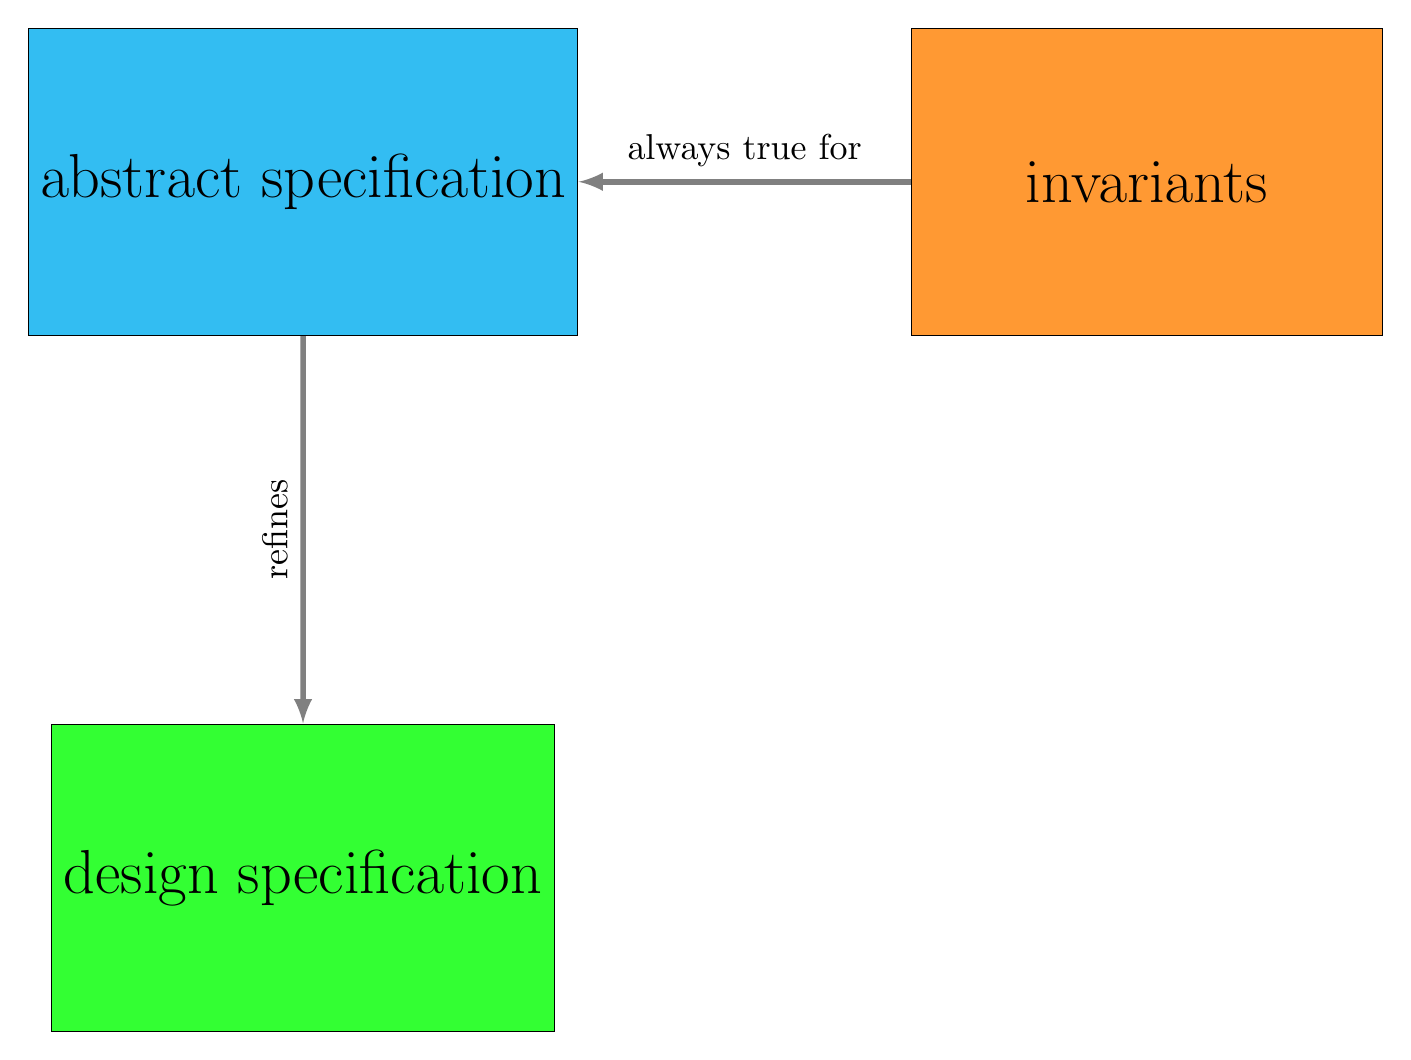
\begin{tikzpicture}[node distance=4cm, every node/.style={scale=1.3}]
        % styles
        \tikzstyle{cell} = [rectangle, minimum width=4.6cm, minimum height=3cm, text centered, draw=black]
        \tikzstyle{arrow} = [line width=2pt,->,>=latex,draw=gray]
        \tikzstyle{box} = [draw, rectangle, align=center, minimum width=11cm, inner sep=3ex]

        % wrap
        \node (abstract) [cell, fill=cyan!80] {\LARGE abstract specification};
        \node (invs) [cell, fill=orange!80, right=120pt of abstract] {\LARGE invariants};
        \node (design) [cell, fill=green!80, below=140pt of abstract] {\LARGE design specification};
        
        % \node [color=red] at (0, -150pt) {blocked access};
        % \node [color=green!200] at (-115pt, -180pt) {good access};

        % flow of information
        \draw [arrow] (abstract) -- (design) node[midway, left] {\rotatebox{90}{refines}};
        \draw [arrow] (invs) -- (abstract) node[midway, above] {always true for};
    \end{tikzpicture}
    \caption{Depiction of the proof architecture explored in this thesis.
    A high-level description of what \lstinline{udp_wrap} should do
    is described in code in the abstract specification.
    An more concrete implementation which makes some assumptions about hardware
    is then defined in the design specification.
    Desirable qualities of \lstinline{udp_wrap} are described as invariants,
    which apply to the abstract specification.
    Lastly, a notion of program correspondence is shown between the
    abstract and design specification---namely, the design specification
    should refine the abstract specification.
    }
    \label{fig:proof-structure-abstract-design}
\end{figure}
The proofs we present in this thesis are structured into 
two overarching divisions: specifications and proofs.
Specifications precisely define how a software works.
In our case, we have two specifications for UDP wrap.
First we have an abstract specification,
which defines the process of prepending a header to a packet of data
in precise terms, but ignoring many implementation details that would
be important for execution on hardware.
Next, we have a design specification,
which describes the same behavior, but using the language of bits and bytes
that is more amenable to hardware.

The two types of proofs we have are invariants and refinement.
An invariant is a property of the abstract specification that should always
be true. These are used to show that our specification does what we want it to
do. In our case, the statement that UDP unwrap should be the inverse of UDP wrap
is an invariant,
since it should always be true regardless of what data is being sent.
Refinement is the process of showing that the design specification 
corresponds to the abstract specification.
Specifically, refinement states that every possible result of the design
specification is an allowed result of the abstract specification.
Since we know from the invariant that the abstract specification 
works the way we want it to, through refinement we know
that the design specification also works the way we want it to.


\section{Abstract specification}
In the abstract specification, we model all fields as natural numbers,
disregarding size.
As such, we transition from thinking about packets of data
(the phrasing of which invites thinking of hardware)
to a more abstract notion of a message,
namely a list of natural numbers (see line 1 of \ref{fig:defs-abstract}).

\begin{figure}[htpb]
    \centering
\begin{nlisting}[language=isabelle]
type_synonym message $=$ "nat list"
type_synonym ip_addr $=$ "nat"
type_synonym port $=$ "nat"
type_synonym socket $=$ "ip_addr $\times$ port"
type_synonym connection $=$ "socket $\times$ socket"
definition src :: "connection $\Rightarrow$ socket" where "src c $=$ fst(c)"
definition dst :: "connection $\Rightarrow$ socket" where "dst c $=$ snd(c)"
\end{nlisting}
    \caption{Basic definitions for our UDP abstract specification.
        Fundamental types in the network stack are defined,
        including messages and connections.
        Additionally, helper functions are provided to facilitate 
        the extraction of source and destination sockets from a connection.}
    \label{fig:defs-abstract}
\end{figure}

Additionally, we define the routing information used throughout the
network stack.
Network communication is done over a connection,
which is uniquely defined by a source and destination socket
(see lines 5,6, and 7 in figure~\ref{fig:defs-abstract}).
A socket consists of an ip address and a port (line 4 of figure~\ref{fig:defs-abstract}), both of which are again natural numbers.

We define the abstract UDP wrap using the pure function approach:
UDP wrap should take in a message from the application layer above,
then use information about the connection to create a header.
Finally, UDP wrap will output a new message, which consists of the header
prepended to the old message, to be sent to the IP layer below.
The precise definition is shown in figure~\ref{fig:wrap-abstract}.

\begin{figure}[htpb]
    \centering
\begin{lstlisting}[language=isabelle]
definition udp_wrap :: "message $\Rightarrow$ connection $\Rightarrow$ message" where
  "udp_wrap msg conn $\equiv$ (let
                          src_sk $=$ src conn;
                          dst_sk $=$ dst conn;
                          src_ip_addr $=$ ip_addr src_sk;
                          dst_ip_addr $=$ ip_addr dst_sk;
                          src_port $=$ port src_sk;
                          dst_port $=$ port dst_sk;
                          len $=$ length_octets msg $+$ udp_hdr_sz
                        in
                          [src_port, dst_port, len,
                           checksum16 [src_ip_addr,
                                       dst_ip_addr,
                                       0, udp_proto, len]
                          ]) $@$ msg"
\end{lstlisting}
    \caption{The definition of UDP wrap in the abstract specification.
        The notation used here serves to say that \lstinline{udp_wrap}
        is a nonrecursive function that takes two arguments:
        a message \lstinline{msg}, and a connection \lstinline{conn},
        and outputs a new message.
        The function creates the header from the connection information,
        and then returns
        the header, presented as a list of computed natural numbers,
        appended via that $@$ operator with the input message
        \lstinline{msg}.
    }
    \label{fig:wrap-abstract}
\end{figure}

Some features of this implementation of the specification bear mentioning.
First, as specified by RFC 768, the length field (depicted in figure~\ref{fig:udp-wrap-rfc}) should be the total size of the output message in octets.
This is not necessarily the length of the message itself,
since the message is expressed as a list of natural numbers, rather than
a list of octets.



\section{Design specification}
The design specification proceeds very similarly to the abstract specification,
but with all fields defined in terms of bytes or 16-bit words rather than
natural numbers, as seen in figure~\ref{fig:defs-design}.
Words are defined here using the Isabelle Word library
(TODO: citation needed).

\begin{figure}[htpb]
    \centering
\begin{lstlisting}[language=isabelle]
type_synonym message_d = "byte list"
(* IPv6 addresses consist of 8 16-bit words *)
type_synonym ip_addr_d $=$ "word16 $\times$ word16 $\times \cdots \times$ word16"
type_synonym port_d $=$ "word16"
type_synonym socket_d $=$ "ip_addr_d $\times$ port_d"
type_synonym connection_d $=$ "socket_d $\times$ socket_d"
\end{lstlisting}
    \caption{Basic definitions for our UDP design specification.
    Fundamental types in the network stack are defined
    in terms of bytes and 16-bit words.
    Omitted here for the sake of brevity are most of the 16-bit words
    that make up an IPv6 address---in the true Isabelle specification,
    all 8 16-bit words are listed.}
    \label{fig:defs-design}
\end{figure}

Worthy to note here is that many fields are too large to fit into
a single atom of the message, since the message consists of a list of
8-bit bytes, while a port consists of a 16-bit byte, and
an ip address spans a total of $16*8= 128$ bits.
This means that some additional helper functions are needed
to split up ip addresses and ports into byte-sized pieces.
The function for ports is displayed in figure~\ref{fig:porttomsg-design}.

\begin{figure}[htpb]
    \centering
\begin{lstlisting}[language=isabelle]
definition porttomsgd :: "port_d $\Rightarrow$ message_d" where
  "porttomsgd p $=$ [w16tow8h p, w16tow8l p]"
\end{lstlisting}
    \caption{Function to convert a 16-bit port to a message
        consisting of 8-bit words.
        This conversion is done by listing first the 8
        most-significant bits of the port, followed by
        the remaining 8 less-significant bits.}
    \label{fig:porttomsg-design}
\end{figure}

The definition for UDP wrap in the design specification is
again very similar to the definition in the abstract specification.
One of the more notable differences is 
that rather than expressing the header as a list of natural numbers,
we must instead express it as result of several list appends,
as seen in lines 13 through 17 of figure~\ref{fig:wrap-design}


\begin{figure}[htpb]
    \centering
\begin{nlisting}[language=isabelle]
definition udp_wrap_d :: "message_d $\Rightarrow$ connection_d $\Rightarrow$ message_d"
where "udp_wrap_d msg conn $\equiv$ (let
                            src_sk $=$ src conn;
                            dst_sk $=$ dst conn;
                            src_ip_addr $=$ ip_addr src_sk;
                            dst_ip_addr $=$ ip_addr dst_sk;
                            src_port $=$ port src_sk;
                            dst_port $=$ port dst_sk;
                            len $=$ (of_nat
                        (length msg $+$ udp_hdr_sz)::word16);
                            chksum $=$ (0 :: word16)
                          in
                            (porttomsgd src_port $@$
                             porttomsgd dst_port $@$
                             w16tomsg len $@$
                             w16tomsg chksum
                            ) $@$ msg)"


\end{nlisting}
    \caption{The definition of UDP wrap in the design specification.
        Again, we construct the header from the connection information,
        then return the header appended with the input message.
    }
    \label{fig:wrap-design}
\end{figure}

Notice that since here we have already formatted the message as
a list of bytes, we can simply take the length of the message
to compute the length field.



\section{Invariants}
We present all invariants as Hoare triples, which is a 
statement on a state-transforming imperative program.
Hoare triples are of the form shown in figure~\ref{fig:hoare-triple-structure},
and consist of a precondition, a terminating program, and a postcondition.
In this context, a program is defined as in figure~\ref{fig:prog-def-det-nondet},
and takes as input an initial state, executes some computations, then returns
an output state.
In this context, the precondition operates on the initial state, while the 
postcondition operates on the final state.

\begin{figure}[htpb]
    \centering
    % TODO: some weird line breaks caused by the color boxes
\begin{lstlisting}[language=isabelle]
lemma "
&\color{green!200}{\{precondition\}}&
&\color{cyan!200}{program that changes state}&
&\color{blue!180}{\{postcondition\}}&
    "
\end{lstlisting}
    
    \caption{Structure of a Hoare Triple.
        This statement is read as
        ``assuming {\color{green!200}precondition} is true,
        and {\color{cyan!200}program that changes state} is a terminating
        program, then {\color{blue!180}postcondition} is true.
        }
    \label{fig:hoare-triple-structure}
\end{figure}


In this thesis, we have focused on defining the UDP wrap functionality,
and have not discussed the UDP unwrap endpoint at length.
Hence, we will provide the statement of an invariant 
that UDP unwrap is the inverse of UDP wrap, but not prove it.
This statement is presented in figure~\ref{fig:inv-unwrap-wrap}.


% TODO: invariant singular?
\begin{figure}[htpb]
    \centering
\begin{lstlisting}[language=isabelle]
lemma compose_to_id:
"VARS orig_msg wrapped_msg unwrapped_msg conn
&\color{green!200}{\{well\_formed orig\_msg conn\}}&
&\color{cyan!200}{wrapped\_msg := udp\_wrap orig\_msg conn;}&
&\color{cyan!200}{unwrapped\_msg := udp\_unwrap wrapped\_msg}&
&\color{blue!180}{\{orig\_msg = unwrapped\_msg\}}&"
\end{lstlisting}
    \caption{Invariant stating that UDP unwrap is the inverse of UDP wrap.}
    \label{fig:inv-unwrap-wrap}
\end{figure}

\begin{itemize}
    \item mention that we can't prove this invariant yet, since we need
        to define unwrap?
    \item give some nice formal definitions of Hoare triples
        from semantics.
    \item discuss how the triples themselves can be composed to get bigger triples
    \item mention that this is from the HOL-Hoare library or whatever
\end{itemize}



\section{Refinement}

\section{Ongoing and future work}
\subsection{Convert C to Simpl}
\begin{itemize}
    \item show some example conversions
    \item discuss need to switch to more seL4 way of doing things?
\end{itemize}

\chapter{Conclusions}
\section{Conclusions}
\section{Future Work}
\begin{itemize}
    \item Make abstract and design specs for other layers
    \item c conversion for other layers
    \item c conversion for UDP?
    \item refinement for other layers
    \item seL4 proofs (specifically, PD stuff)
    \item introduce hardware problems
        \begin{itemize}
            \item think of this as relaxing assumptions about hardware
            \item e.g. packets won't be corrupted, but could arrive in weird orders
            \item note that there's probably a limit to this,
                since a packet could randomly corrupt to
                look completely legit---it's just very
                unlikely with all the error correction
                going on.
                Thus, we could model this by, e.g.,
                saying that only a limited arbitrary subset
                of the packet can be corrupted;
                or by saying any part of the packet other
                than the CRC can be corrupted.
                Pros/cons to each.
        \end{itemize}
    \item introduce linear temporal logic to have some ``always eventually''-type stuff
\end{itemize}
\section{Discussion}

\chapter{A Day in the Life of}
\begin{itemize}
    \item some isabelle guidelines
\end{itemize}


\section{Isabelle session management}
TODO: where to put this? Appendix?
At the root of your directory tree, a ``ROOTS'' file may be placed, which describes all directories with required sessions (see figure~\ref{fig:isabelle-roots-file}).
Each directory referred to in the ROOTS file must contain a ``ROOT'' file, which provides isabelle with the information for creating various sessions
(see figure~\ref{fig:isabelle-root-file-spec}).
Sessions in a particular ROOT file may refer to sessions in another, but with some restrictions.
In our example, the refinement session RefineAD deals with the abstract and design specifications, whose theories are contained in sessions
ASpec and DSpec.
Hence, our ROOTS file must contain a reference to both parent directories spec/ (which contains the files for both ASpec and DSpec), and proof/
(which contains the files for ADRefine).
Furthermore, the ADRefine session must explicitly list ASpec and DSpec as required parent sessions in its own ROOT file under proof/ (see figure~\ref{fig:isabelle-root-file-proof}).

\begin{figure}[htpb]
    \centering
    \begin{lstlisting}[style=tree, language=file]
    .
    ├── README.md
    ├── ROOTS
    ├── proof
    │   ├── InvsA
    │   │   └── UDPInverse.thy
    │   ├── ROOT
    │   └── RefineAD
    │       ├── Corres.thy
    │       └── RelationUdp.thy
    └── spec
        ├── Aspec
        │   ├── Network_A.thy
        │   └── Udp_A.thy
        ├── Dspec
        │   ├── Network_Consts.thy
        │   ├── Network_D.thy
        │   ├── Udp_D.thy
        │   └── Word_Network.thy
        └── ROOT
    \end{lstlisting}
    
    \caption{Example directory structure}
    \label{fig:isabelle-roots-file}
\end{figure}

\begin{figure}[htpb]
    \centering
    \begin{lstlisting}[language=isabelle]
session ASpec in "Aspec" = HOL +
  theories
    "Network_A"
    "Udp_A"

session DSpec in "Dspec" = HOL +
  sessions
    "HOL-Library"
  theories
    "Network_D"
    "Udp_D"
    \end{lstlisting}
    
    \caption{Example ROOT file in the spec/ directory. Two sessions are created: ASpec (an abstract specification) and DSpec (a design specification).}
    \label{fig:isabelle-root-file-spec}
\end{figure}

\begin{figure}[htpb]
    \centering
    \begin{lstlisting}[language=isabelle]
session RefineAD in "RefineAD" = HOL +
  sessions
    "ASpec"
    "DSpec"
  theories
    "Relation"
    \end{lstlisting}
    
    \caption{Example ROOT file in the proof/ directory. Note that the RefineAD session relies on the ASpec and DSpec sessions defined in a different ROOT file (in our case, located in the spec/ directory).}
    \label{fig:isabelle-root-file-proof}
\end{figure}


% If you want to include appendices, just use the \appendix command and then make chapters as normal
\appendix
\chapter{Installation notes}

See \url{https://www.overleaf.com/read/qyhckhfyfvmb} on Overleaf for useful examples of formatted text, typing in IPA, etc.

% For the bibliography style, I load `sp.bst', the style used by the LSA in the journal `Semantics and Pragmatics'. For how to include in-line citations with page numbers and other conventions, refer to nus-el-ht.sty. 
\backmatter
\bibliography{el-ht.bib}
\end{document}

